\chapter{Poroelastic natural coatings}

\chapquote{Nature is the source of all true knowledge. She has her own logic, her own laws, she has no effect without cause nor invention without necessity}{}{Leonardo Da Vinci}

\section{Biomimetics of poroelastic coatings}

Usually when someone is asked to imagine some "rapid" object as an airplane, a boat or a car, the common sense lead us to think about it as the smoothest as possible.
But if we look around, nature seems not to agree with the previous statement.
In fact most of the surfaces in nature are not smooth at all, they almost always present some kind more or less regular arrangement of discontinuities at various length scales.
Since Nature have had a very large time-span to optimize this kind of surfaces we can be very certain that they are the best possible option.
One should pinpoint that the non smoothness of these surfaces can be connected to some other biological functions rather than pure fluid dynamic performance, and of course it can be the case.

With that in mind we want to show the reader some of the most notable examples of "natural" aerodynamic surfaces.

Probably the most notable example is the shark skin, in figure \ref{fig:shark} a segment of the skin is depicted, as if appears to be, under the microscope.

\begin{figure}[h]
	\centering
	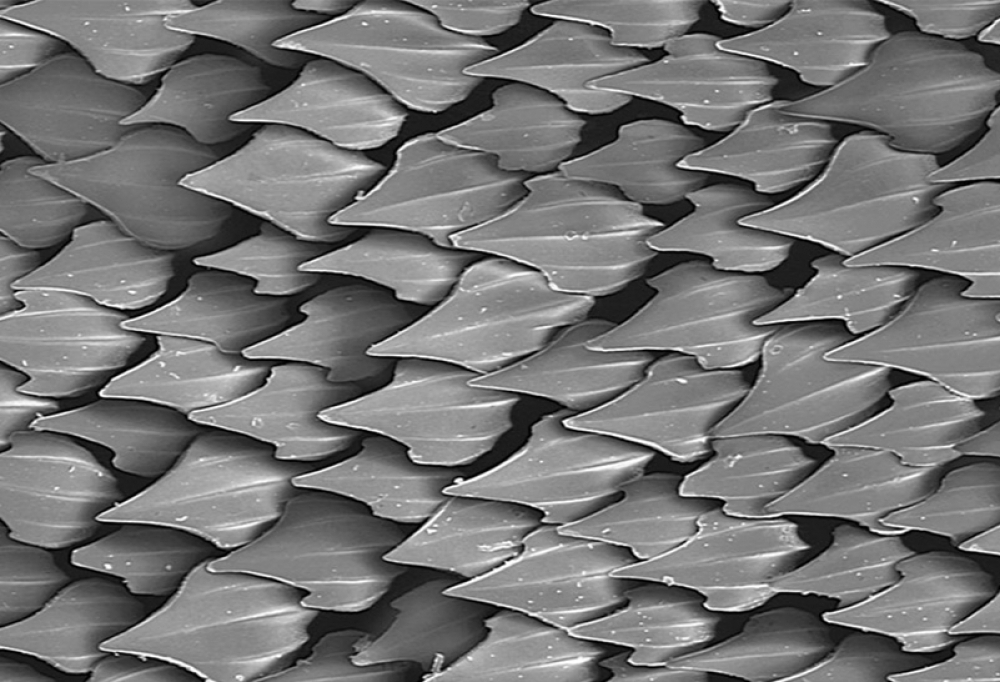
\includegraphics[width=0.6\linewidth]{chapter_1/shark}
	\caption{Microscope enlarged picture of the shark skin}
	\label{fig:shark}
\end{figure}

The enlargement show that the surface is made up by a series of overlapped denticles, and experiment shows that they can move and interact with the flow.

The shark "technology" has somehow been applied by Speedo$^{\circledR}$; they have fabricated their famous swimming suits with a surface that mimic the roughness of sharks; and they happen to break multiples world records.
But it seems that this controversial swimmers performance was due to the fact that they compress the body giving the swimmer a more and streamlined shape.
But even thought the company has been publicized their product as it was a synthetic shark skin, \citet{Oeffner785} has shown that the texture of their swimming suits is somehow different from the shark dermal structure.
In they work the authors have performed swimming experiment with a flat plate with different surfaces and they did not found significant speed enhancement with the swimsuit surfaces; but the measurements with real shark skin on the contrary give an appreciable improvement in the performance.


Poroelastic surfaces find also applications in aeroacoustics, in fact owls are well known for their particularly silent flight, especially in the high frequency spectrum.
This characteristic is crucial for the owl in order to be able to capture his preys.
Obviously it has inspired the scientific community to study their feathers configuration and shape.

\begin{figure}[h]
	\centering
	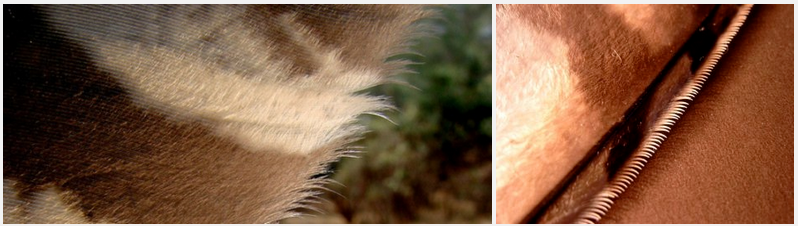
\includegraphics[width=0.8\linewidth]{chapter_1/howl}
	\caption{Feathers in owl's wing. Left: trailing edge. Right: leading edge. The difference in shape, mechanical properties, as rigidity, between the leading and trailing edge is a consequence of the different flow regimes in the wing}
	\label{fig:owl}
\end{figure}
 
Multiple authors show promising result in characterizing the acoustic properties of the owl skin and their physical mechanism.
In particular \citet{lilley1998} present three main characteristic of the owl that can suppress its airborne noise: the feathers leading edge shaped like a comb; the trailing edge that form a fringe, and the presence of multiple "filaments" in the bottom surface of wing and legs.
In the same work the authors also present some experimental and empirical evidence on the aeroacoustics mechanism behind the three elements above.

Another example of work in the field of owls acoustic is the one by \citet{jaworski2013aerodynamic} in which the authors study the acoustic scattering problem of a poroelastic half-plane hit by an incident plane wave.
This configuration has been used as an analogy with the owl wing, it try to explain how the properties of this surface can suppress the noise.
They conclude that the combined effects of elasticity and porosity can produce weakest noise amplification.

Recent computational simulation made by \citet{rao2017owl} confirm that the leading edge shape of the feathers truly suppress noise and enhance the lift generation.

Bioinspired aerodynamic surfaces include another peculiar example in the butterflies wings.
In figure \ref{fig:butterfly} the surface of a "Peacock butterfly" is enlarged in order to show the multiple scales involved; the wing structure present firstly a series of overlapped scales similar to the shark, but looking closely we can observe that the singles scales have a complicated permeable structure.

\begin{figure}[h]
	\centering
	\begin{subfigure}[b]{0.3\textwidth}
		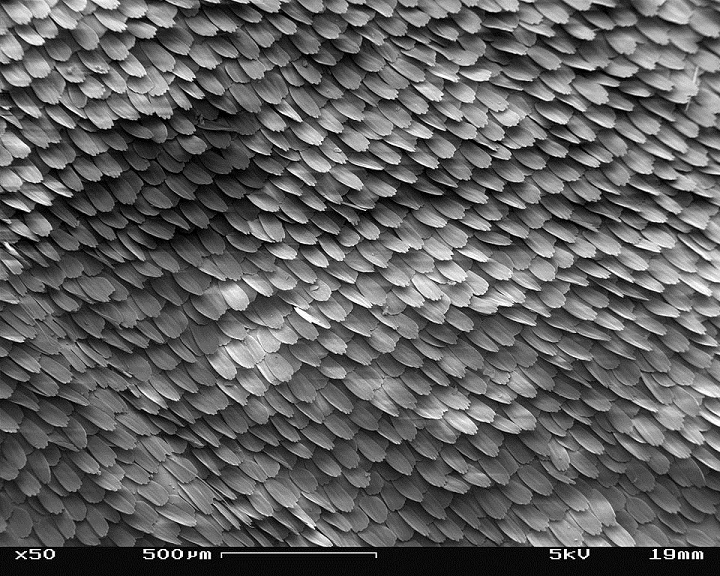
\includegraphics[width=\textwidth]{chapter_1/butterfly}
		\caption{Magnification 50x}
		\label{fig:b50}
	\end{subfigure}
	~ %add desired spacing between images, e. g. ~, \quad, \qquad, \hfill etc. 
	%(or a blank line to force the subfigure onto a new line)
	\begin{subfigure}[b]{0.3\textwidth}
		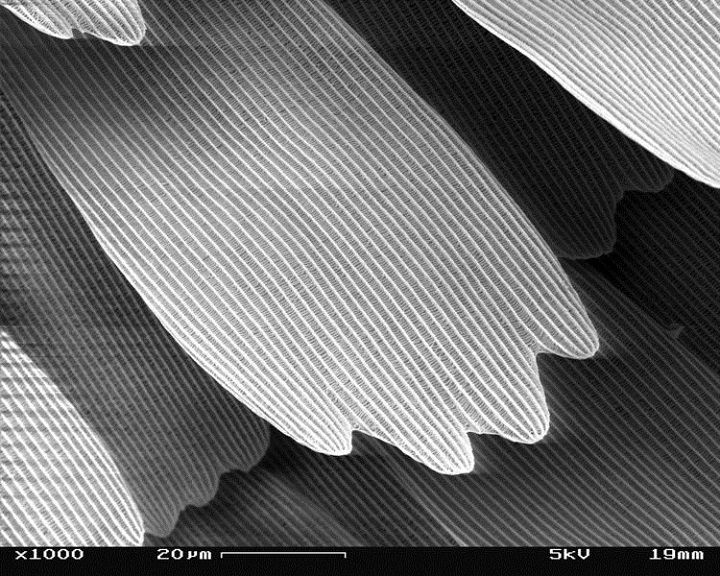
\includegraphics[width=\textwidth]{chapter_1/butterfly2}
		\caption{Magnification 1000x}
		\label{fig:b1000}
	\end{subfigure}
	\begin{subfigure}[b]{0.3\textwidth}
		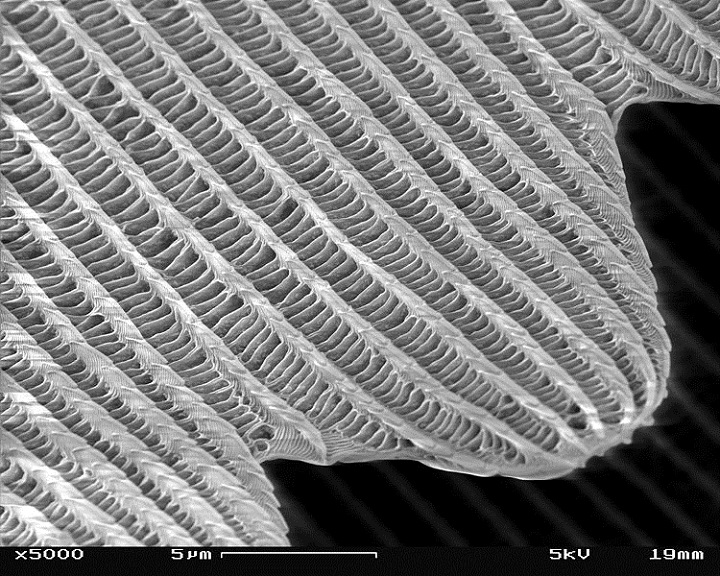
\includegraphics[width=\textwidth]{chapter_1/butterfly3}
		\caption{Magnification 5000x}
		\label{fig:b5000}
	\end{subfigure}
	\caption{Peacock butterfly wing surface using Scanning Electron Microscopy.  Images from wikimedia.org}
	\label{fig:butterfly}
\end{figure}

The work of \citet{slegers2017beneficial} study the effect of such porous structure in the flight performance of butterflies.
Using cameras to measure the kinematics of their flight, they can compute their efficiency to "climb" (generate lift) and the stroke amplitude and frequency.
The authors conclude that the porous structure of their wing gives a boost in climbing efficiency about $30\%$; that result clearly stress out the importance of poroelastic layer coating of the wings. 
Even though the butterfly flight aerodynamic is extremely complex, it seems clear that the peculiar structure of the wings surface is critical for their aerodynamic performances \citet{srygley2002unconventional}.

The last example will be super-hydrophobic surfaces; these surfaces are water repellent, it means that the water can slide over with much less resistance resulting in very small values of wettability.
This behavior is caused by the microscopic structure that forms the surface (see figure \ref{fig:lotus}), in fact the rugosities are arranged in a more or less regular ways in order to be able to capture air pockets that rest inside this structures.
These air inclusions provoke an effective slip at the air-liquid interface that cause the drag reduction; they also change the contact angle of droplets.
The work of \citet{bottaro2003effect} summarize the above aspect and their applications.

\begin{figure}[h]
	\centering
	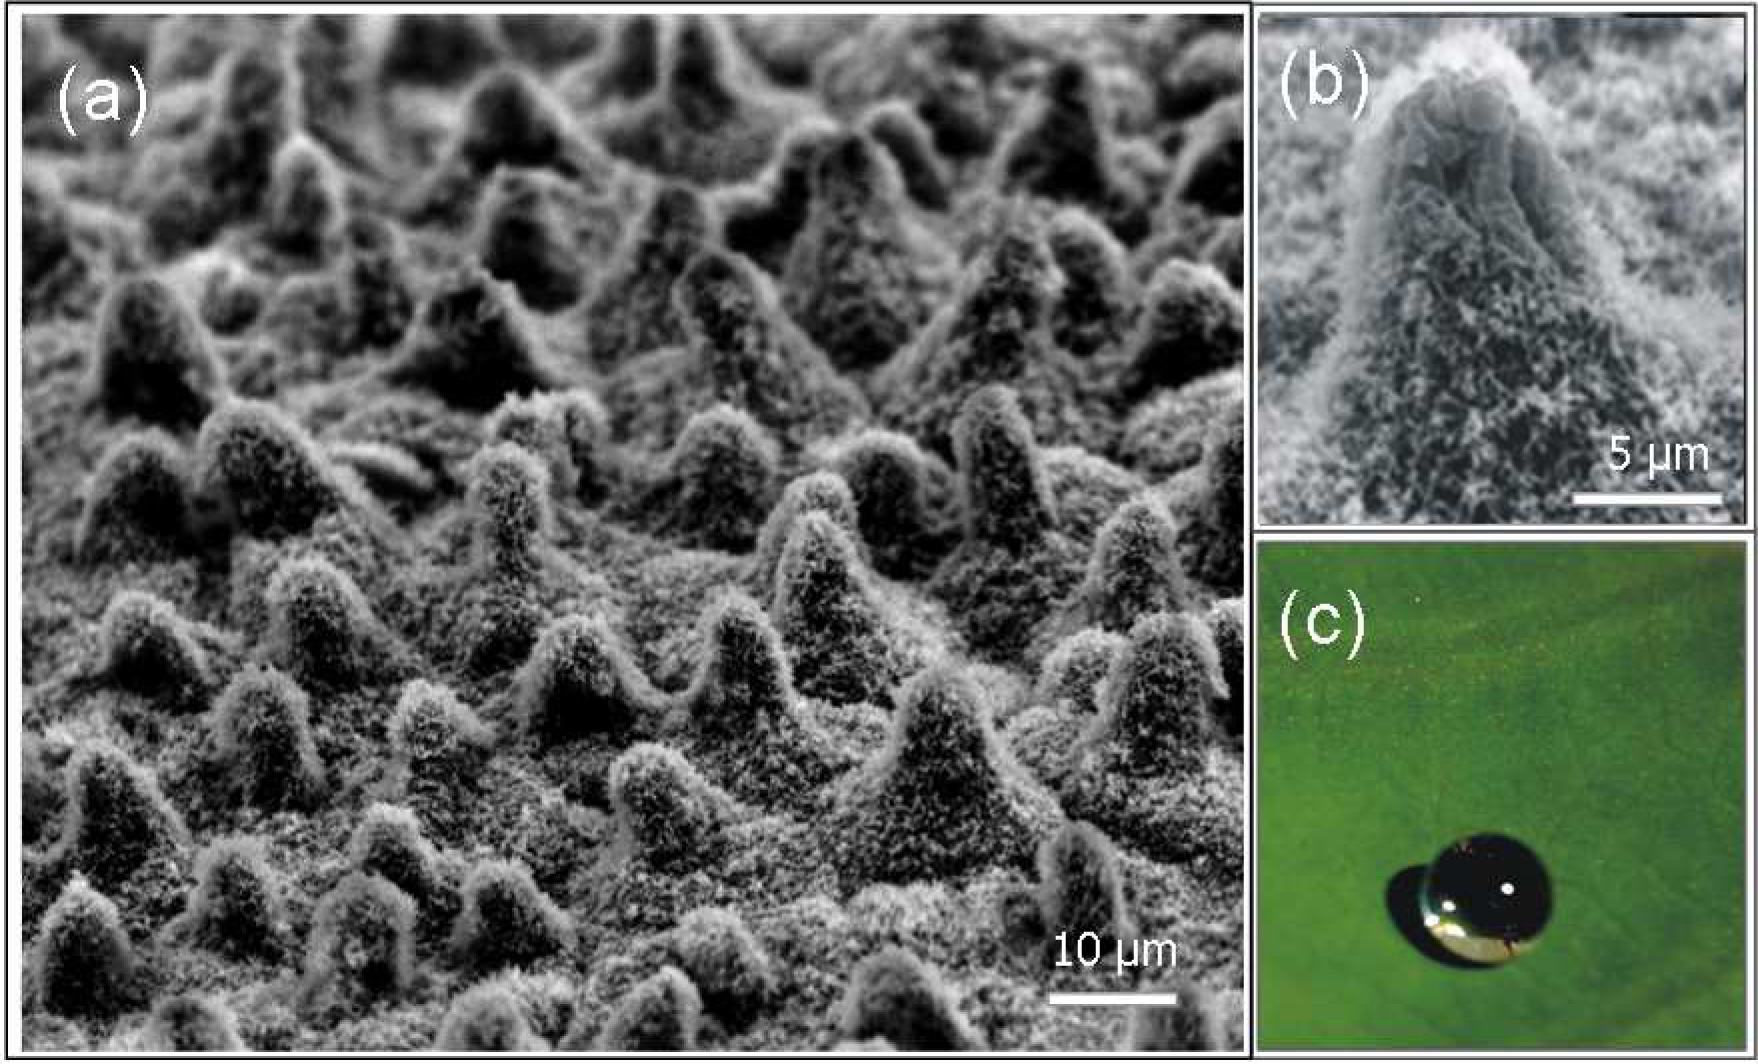
\includegraphics[width=0.6\linewidth]{chapter_1/lotus}
	\caption{(a) Scanning electron microscopy (SEM) image showing the structure of lotus leaf, (b) higher order of magnification on the single protuberance forming the surface and (c) a water drop that due to the contact angle attain an almost spherical shape. Images from \citet{stratakis2009laser}}
	\label{fig:lotus}
\end{figure}

The interest reader could find other examples and broaden the above key aspect in \citet{bhushan2016biomimetics}, \citet{tropea2012nature}.

\subsection{Riblets and shark-skin surfaces}

We have seen that natural surface can be an inspiration to find strategies in solving many aerodynamics problems; in the following we will focus especially on the drag reduction.

Is known that the total drag contribution can be separated in different components, and the classical decomposition is between viscous drag (sometimes referred as skin friction) and pressure drag.

\begin{equation}
 \int_{A_{\sigma}}  [ \underbrace{\left( \frac{p}{\rho} \mathbf{I} \right) \cdot  \mathbf{n}_{\sigma} }_\text{pressure drag}  +  \underbrace{ \left( \nu \nabla \mathbf{v} \right) \cdot  \mathbf{n}_{\sigma}}_\text{viscous drag} ] \; dA,
 \label{eq:force}
\end{equation}

In \eqref{eq:force} $A_{\sigma}$ is the solid interface of some body where a no slip condition is applied, and $ \mathbf{n}_{\sigma}$ is its outward normal.
This section will talk about the existing ways to reduce the viscous part of the drag since historically has attracted more interest and/or make more progress.

In the following we will refer as the wall shear stress in the turbulent case as:

\begin{equation}
\tau = \left( \left( \mu + \mu_t \right)  \nabla \mathbf{\overline{v}} \right) \cdot  \mathbf{n}_{\sigma} = \left( \mu + \mu_t \right) \derp{\overline{u}}{y}
\end{equation}

where $\mu_t$ is the turbulent viscosity and $\overline{u}$ is the average velocity stream-wise component; in the laminar case obviously the definition rest the same with the appropriate corrections (there is no turbulent viscosity and no notion of average velocity).

Most of the industrial application involves turbulent flow; obviously there is a lot of research that aim to reduce the skin-friction in this regime.
Table 6.3.1 in the book of \citet{mclean2012understanding} make a wide list of technique already been proposed on the problem.

As the same author pinpoint, the most effective and, probably the most practicable concept are the riblets.
Riblets are alternating ridges aligned in the stream-wise flow direction and regularly arranged as the figure \ref{fig:riblets1} show.

These surfaces are capable of align the turbulent flow in the mean flow direction smoothing the fluctuation of the cross-flow in the viscous sublayer.
Reducing this fluctuations close to the surface the turbulent momentum transfer will also be reduced and so the shear stress, causing the reduction in skin-friction.

\begin{figure}[h]
	\centering
	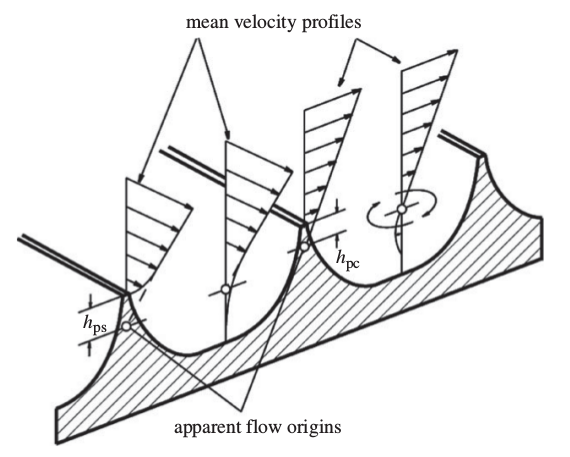
\includegraphics[width=0.7\linewidth]{chapter_1/riblets3}
	\caption{Schematics of the  \textit{protrusion height} concept. The mean velocity profiles for the stream-wise and cross-flow velocities are shown. In presence of a ridge is it possible to extrapolate the point of zero velocity from the velocity gradient outside the riblet; finding respectively, the \textit{stream-wise protrusion height} $h_{ps}$ and the \textit{cross-flow protrusion height} $h_{pc}$. Image from \citet{bechert1997experiments}}
	\label{fig:riblets1}
\end{figure}

The viscous drag reduction correlates well with the spacing between the ridges expressed in wall units $ s^+ $; the typical shape of the latter relation is depicted in figure \ref{fig:riblets_perf}, where the vertical axis show the drag reduction against the $ s^+ $.
This general shape of the curve, in which the skin friction decrease in certain range of spacing and then increase as the ridge spacing  increase, is caused by a competition between the capacity of riblets to obstruct lateral fluid flow and an increase in the penetration of high speed vorticies inside this manufactured rugosities.

\begin{figure}[h]
	\centering
	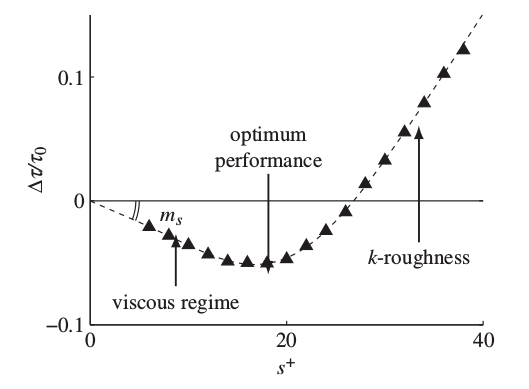
\includegraphics[width=0.5\linewidth]{chapter_1/riblets_performance}
	\caption{Example of drag reduction relation to the ridge spacing. The maximum performance is normally around $ s^+ = 15 $, the picture show also that when the riblet are really tight one another the laminar case is retrieved. On the contrary when the riblets are far away one other their performance is comparable to rough plate case. Image from \citet{jimenez2001turbulent} }
	\label{fig:riblets_perf}
\end{figure}

This last physical explanation of the riblets performances is presented in the schematics \ref{fig:riblets_schem}, where the gray areas show high skin-friction regions caused by the down-wash motion generated by the near-wall vortices.
Is it clear that when the riblets are too big the vortices can penetrate inside its groove, and actually increase the skin-friction due to larger area exposed to the local velocity.
On the contrary when the riblets are smaller, the high speed vortex "touches" only the tip of the ridges so only a small local area of the surface experience high-shear stresses.

\begin{figure}[h]
	\centering
	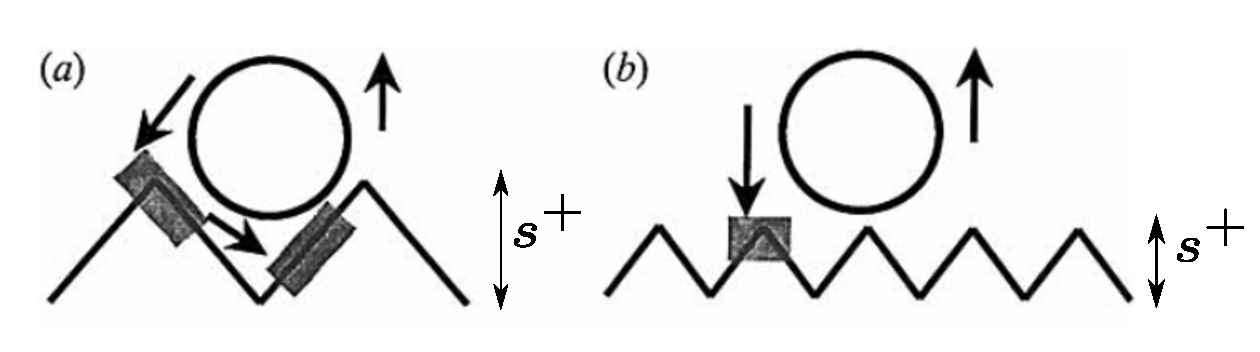
\includegraphics[width=0.7\linewidth]{chapter_1/riblets1}
	\caption{Two different size of riblets are shown when interacting with a sublayer vortex. In gray is it represented the areas where friction is important. Clearly when the size of two is comparable the surface experience a larger friction and the performance is lowered. Image from \citet{choi1993direct}}
	\label{fig:riblets_schem}
\end{figure}

The slope $m_s$ of the curve in figure \ref{fig:riblets_perf} can be predicted by linear stability theory or by means of empirical correlations \citet{garcia2011hydrodynamic}.

Computing the performance of such surfaces can be expensive since the most reliable quantitative theory for such problems are direct numerical simulations (DNS) or experiments.
There is only one other theory, besides the already cited expensive ones, that use the concept of \textit{protrusion height} showed in figure \ref{fig:riblets1} to correlates the shape of this protrusion to the drag reduction \citet{luchini1991resistance}.
The \textit{protrusion height} is defined as the vertical distance between the riblet top ridge and point of zero velocity extrapolated from the constant velocity gradient outside above the protrusions.
It seems that especially the difference of protrusion heights, computed from the stream-wise $h_{ps}$ and cross-flow flow $h_{pc}$ profile, correlates very well with the drag reduction, and the two quantities can be computed with a simple Stokes problem over the local geometry of the grooves.
The last results has been analyzed by \citet{segura2017permeable} that came out with an empirical law for the drag reduction, that relates the previous protrusion heights with the permeability expressed in wall units:

\begin{equation}
DR \approx 0.04\left( \sqrt{{K^+}_s} - \sqrt{{K^+}_c} \right),
\label{eq:max_dr}
\end{equation}

where ${K^+}_s$ and ${K^+}_c$ are the stream-wise and cross-flow permeability tensor components.
This law establish an instrument to estimate the drag reduction from a given geometry of the wall (the permeability tensor can be computed within the porous media homogenization approach as chapter \ref{ch:vans} will explain).

Another important characteristic of riblets performance is that they are robust in off-design conditions, such as in presence of yaw (misalignment between flow and riblets ridges) and tip ridges erosion \citet{garcia2011drag}.

But still, besides some very specific application such as sailing competitions (the hulls of the USA challengers in the America’s Cup 1987 and 2010), the massive utilization of this technology is still in question.
Producing such surfaces in a larger area, like the roof of a car or the wing of an airplane, can be an issue for a routine use; because riblets size need to be very little to be effective.

Riblets like surface has been observed in nature for many years, for example \citet{Martin2016riblets} found out that skimmer birds (Rynchops) have riblets like grooves in their beak, since they fly with it under the water surface to catch fishes.
However, as already introduced, the most clear example of such natural surfaces are shark skin.
In his review \citet{dean2010shark} present the status of the shape optimization that has been done on the riblets trying to mimic the typical sawtooth shape seen in shark skin, showing that improvements of such geometries over the classical ones has yet to be proven.
Shape optimization on riblets geometry has been studied, the findings show that just a few $\%$ can be improved on the base line geometry \citet{bechert1997experiments}.

There is in fact some controversial result in literature stating that surfaces with actual shark skin replica can indeed increase drag.
\citet{boomsma2016direct} perform some simulations on actual shark skin denticles using the immersed boundary method; the authors find that in some configuration the actual drag increase up to $40\%$, but even though their numbers are probably too large (it is know that the immersed boundary method can generate some errors especially in computing forces at high Reynolds number), this can be a clue that the shark skin does not work with the same mechanism as riblets.

Experiments on such geometries are available in literature \citet{bechert1997natural}.
The authors of the previous work have built a synthetic surface made by artificial shark denticles posed on top of springs and measure that even with the introduction of  surface elasticity the actual drag was increasing.
However the authors pinpoints that the actual shark flow regime is not steady as the experiments that he performed, and they speculate that the excellent swimming performance of the shark came from the separation control that flexible denticles can increase in the periodic oscillating flow that the swimming generate.

Experiment using DPIV on a NACA profile covered with actual skin samples of "Isurus oxyrinchus" mako shark, has been performed by \citet{lang2014SharkControl}, confirming that the flexibility of sharks denticles act as a passive flow control in order to avoid early separation.
In fact the experiments proves that for angles of attack larger than $15^{\circ}$ the flow reversal is almost completely avoided.
The same author introduce the importance in the different geometries of the denticles in various part of the body that obviously experience disparate flow condition,
\citet{motta2012Shark} perform a detailed collection of flexibility and scale measurement of different shark species that can be valuable for future studies.

Swimming experiment from \citet{Oeffner785}, who used a flat plate covered with real shark skin, also confirm the previous flow control mechanism and also make some conjectures about possible thrust enhancing controlled by the same movable scales that can move away the leading edge vortex.

Also \citet{itoh2006turbulent} shows that movable rugosities can outperform riblets, the authors in fact measure the drag reduction of a seal fur (that present fibrous movable surface) against a riblet surface in an experimental channel; its results are show in figure \ref{fig:seal}.

\begin{figure}[h]
\centering
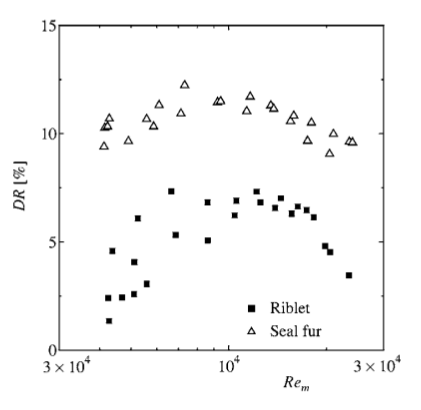
\includegraphics[width=0.5\linewidth]{chapter_1/seal}
\caption{Performance comparison between a riblet surface against a seal fur. The drag reduction has been computed as: $DR \% = \dfrac{ \Delta \tau}{\tau_{0}} \%$ Image from \citet{itoh2006turbulent}.}
\label{fig:seal}
\end{figure}


Compliant surfaces can in fact move accordingly to the surface pressure gradients along the boundary layer and so respond to the pressure fluctuation over the surface itself.
This mechanism is already know to be beneficial in delaying the transition to turbulence and many authors have presented theoretical and experimental evidence on the effectiveness of this solution \citet{carpenter1990status}, \citet{bushnell1977effect}.

In conclusion we have seen that in order to reduce turbulent skin-friction drag, riblets and natural surfaces uses various mechanism such as: sublayer vortices interaction, compliance and separation control.
Such solution have proven to be effective in some cases but they are related mostly in reducing the viscous component of the total drag.
In the next section we will introduce another class of solution that try to act instead mostly on the pressure component.


\subsection{Permeable surfaces}

\subsection{Bluff bodies}

%Permeable surface has been proposed to exploit even further the mechanism explained above using riblets.
There is some experimental evidence that in laminar cases the generation of some \textit{slip velocity}, at the interface between the permeable surface with the fluid, can decrease the friction drag \citet{beavers1967boundary}.
However in the turbulent case it seems that the instabilities developing at the interface can cause an increase in drag up to $40\%$ \citet{jimenez2001turbulent}, \citet{breugem2006influence}; this instabilities mechanism will be further explained in the section \ref{sec:stability}.
Is important to pinpoint that the permeable surface cited in the above references were all rigid.

The pressure contribution to the resistance is usually the most significant one in bluff bodies applications, and even in highly streamlined body it is around $10\%$ of the total drag.
Researchers have tried to find a way to modify the pressure distribution around a bluff body to reduce the associated resistance, and also dump the force oscillation on the body (drag and/or lift).

The pressure drag on a bluff body depends mostly on the difference between the low pressure on the rear part of the body, where there is usually a separated flow region, and the high pressure in the forward part.
This idea is sketched in figure \ref{fig:pressure_dist} where two different pressure distribution are shown; the black one represent the classical solid body, and the green one is the one with a porous layer at the back of the body.

\begin{figure}[h]
	\centering
	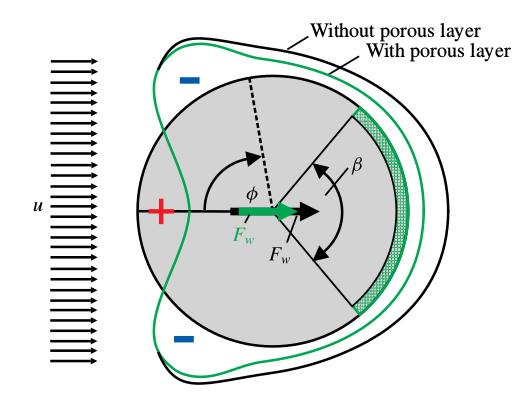
\includegraphics[width=0.4\linewidth]{chapter_1/pressure_dist}
	\caption{Diagram showing an example of angular pressure distribution around a cylinder for viscous flow. The black line is the case of a solid body, the green one is the modified pressure in presence of a porous layer at the rear part. Image from \citet{klausmann2017drag}}
	\label{fig:pressure_dist}
\end{figure}

The favorable increase in the back pressure is due to the low speed laminar flow in the porous media that is ejected in the back region where the separation take place.
Even in very high speed turbulent flow the fluid inside permeable surface exhibit a very high energy loss due to the strong dissipation that the medium provide, resulting in a low speed flow ejected downstream of the body.

The permeable interface, producing a slip velocity, can modify the boundary layer that develops above it and with that produce less shear and vorticity; and can also modify the stability characteristics of the flow.
The instability around a cylinder is due to the shear layer that forms in the top part of the body when the flow start to decelerate.
This shear layer exhibit a Kelvin–Helmholtz type instability that develop in the classical Von-Karman wake.

This two hypothetical mechanisms has been tested by numerical simulation by multiple authors: \citet{bruneau2004passive}, \citet{bruneau2008numerical}, \citet{bhattacharyya2011reduction}, \citet{naito2012numerical}, \citet{mimeau2017passive}.
All these works study the flow around some classical two dimensional bluff bodies (cylinder, square cylinder, Ahmed body section, 3D hemisphere) with the add of a porous layer.

These works show some very promising result on multiple quantities, like: decrease of enstropy, lower oscillations in lift signal, drag reduction, regularization of the wake and lower pressure gradients; even if the porous medium is always rigid in their case.
An example is shown in figure \ref{fig:porous_cylinder} where the turbulent flow field downstream to a square cylinder is shown; the picture show how the porous layer strongly regularize the wake.

\begin{figure}[h]
	\centering
	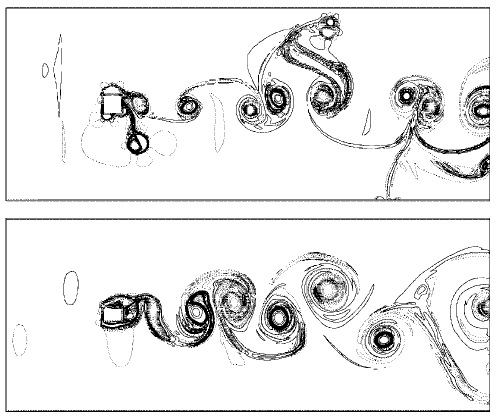
\includegraphics[width=0.7\linewidth]{chapter_1/cylinder_porous}
	\caption{Square cylinder vorticity contour for $Re=30000$. Top: solid case. Bottom: porous case with layer extension $h=10\% D$.}
	\label{fig:porous_cylinder}
\end{figure}


The previous works shows that porous medium parameters, like the medium resistance or its vertical extension, have important effects on the results.
The variety of results seems to agree (at least qualitatively) that increasing the porous medium extension over a certain limit is not beneficial, and they also show that the resistance of the medium should not be excessive in order to be effective (high/medium porosity are the best).

In all these work we also observe: a reduced pressure drop between the front and the rear of the body, a reduced drag, a delays in the vortex shedding and regularization on both the frequency and amplitude of shredded vorticies oscillations.

These works show very optimistic results, but they should be taken with some care; only few cases are three-dimensional, they all use a modeling approach for the porous medium based on a simplified version of the VANS (Volume Average Navier-Stokes equations, see section \ref{sec:vans}) without performing any validation of the method.
Sometimes they also use the equations outside their field of validity (there is some discussion in the scientific community in using the previous version of VANS equations for highly turbulent flows).

The lack of validation reflect the fact that reliable experiment of such porous coatings are almost non existent in literature.
There is also some confusion in literature on how to compute the forces on such bodies surrounded by a porous coating, this differences has taken some authors as\citet{naito2012numerical} to over-estimate the forces and their prediction are not inline with the literature.
There is some theoretical base \citet{caltagirone1994interaction} that establish that the approach used by \citet{bruneau2004passive} is the correct one for that specific version of the VANS used by all the previous authors, REFERENCE TO SECTION IN THE VANS CHAPTER WHERE THERE IS THE FORMULA TO COMPUTE FORCES.

The approach by \citet{favier2009passive} differentiate itself from the previous works, the authors uses a numerical method that includes the dynamic of a moving porous medium made of fibers at the back of a cylinder.
Their results in a laminar flow case agree with the prediction of a stabilization of the wake and show some more realistic values of drag reduction, about $15\%$.
The difficulties in this approach is that the medium dynamic introduces many mechanical parameters that are not easily identifiable for natural surfaces.

A similar model has been used by \citet{venkataraman2012numerical}; the authors applied a movable porous coating in the top part of NACA airfoil.
In this case the synchronization between the oscillations of the structures and the natural frequency of the fluid is responsible for the pressure distribution modification.
They have shown the robustness of this solution in a wide range of angle of attack, in the best case they have found some lift enchantment and a drag reduction around $10\%$.

Later on \citet{rosti2017pelskin} works on a similar configuration with only one movable flap on the low pressure side of airfoil; the results both numerical and experimental qualitatively agree (on the flow mechanism) with the results in the complete porous case.

WHEN IT WILL BE PUBLISHED SHOW SOME RESULTS ON THE 3D SPHERE USING HOMOGENIZATION \citet{zampogna2017new}

The very few experiment in literature on this porous coatings, shows less promising results associated to drag reduction.

For example \citet{heenan1998passive} perform an experiment in which they take a backward facing step with a porous insert in the re-circulation region.
His measurement show a $13\%$ decrease of the peak of pressure at the wall and a relocation of the detachment point further downstream.
A maximum of $9\%$ of drag reduction was observed.
The effect of adding a porous surface in this case was to limit the pressure fluctuations that causes the re-circulation bubble unsteadiness.

Later \citet{klausmann2017drag} study a 3D cylinder with a porous insert in the back (as in figure \ref{fig:pressure_dist}); the authors use a wind tunnel testing with pressure measurements around the body and particle image velocimetry (PIV) flow capture.
Their results confirms that the porous layer on the leeward side increase of pressure in that zone, causing the reduction of drag.
The drag reduction measured was around $10\%$ over various Reynolds number (in turbulence range), this value was sensible to the geometrical parameters of the medium as the position and its size.
At our knowledge this is the first example of actual measurements of flow quantities using PIV, that can later be used to perform some validation on different numerical models.

Some other experimental data can be found in the case of flow over aquatic canopies \citet{zhang2011exchange}, \citet{segalini2011experimental}, \citet{hamed2017impact}, even though the published data is limited and the experiments have the presence of a free surface that increase the difficulty of the problem and limits the possible use as simple validation.

From this section the main physical mechanism that are tied to permeable surfaces has been introduced.
Even thought the different approaches in literature seems to be discordant in the predicted values of some fundamental items such as the forces, a general trend on all the data shows that porous coatings can be effectively used in many situations.
Is it clear that the scientific community need much more experimental data in order to develop new and improved numerical and theoretical models for such permeable coatings.

\subsection{Canopy flow}

Another important class of flow over poroelastic carpets are the \textit{canopy flow} as named in literature.
These type of problems involve flow over flexible slender structure such as threes and aquatic vegetation.
The importance of winds over plants is very important in a large variety of fields, like: the transport of substances as $CO_2$ and nutrients or preventing agricultural damage (wind-throw of crop fields); also some similarities with urban canopies can be found \citet{ghisalberti2009obstructed}.

The boundary layer profile over such canopies differ substantially from the rough wall one, as figure \ref{fig:spectra} shown.
The vegetation resistance cause the creation of an inflection point in the mean velocity profile that lead to a mixing layer type of instability near the vegetation top.
As a consequence of such instabilities \citet{finnigan2000turbulence} show that the vegetation can heavily modify the turbulence spectra as a results of the interface instabilities and the coherent structures above it.
The two bottom pictures in figure \ref{fig:spectra} outline the above statements; the spectrum in case of canopy flow present a larger peak in the frequency of the mixing layer instability, a steeper slope in the energy cascade part due to the larger dissipation inside the permeable layer and possible high frequency peaks associated to the swinging of the pants that can emit or absorb small scales vorticies.
 
\begin{figure}[h]
	\centering
	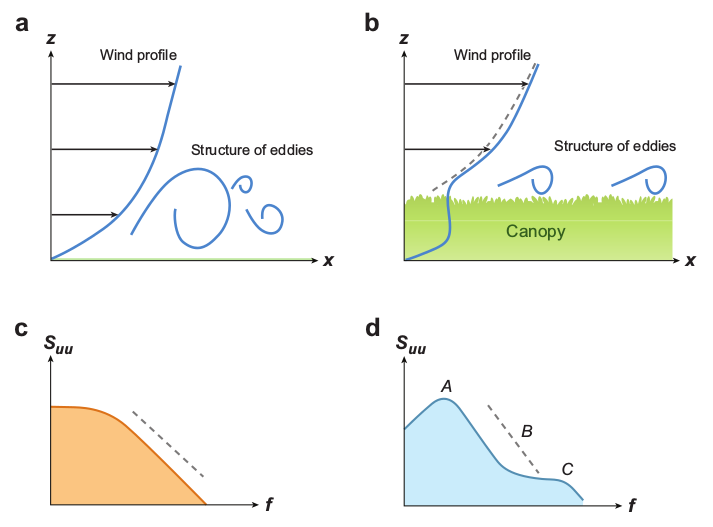
\includegraphics[width=0.7\linewidth]{chapter_1/spectra}
	\caption{Figure \textbf{a} and \textbf{b} show respectively the schematics of the mean flow over a rough wall and a canopy flow; the difference in the eddy size is clear, also the inflection point in the canopy flow velocity profile is transparent.
		The figure \textbf{c} and \textbf{d} instead show the turbulent spectra for the two different flow above, in case of rougth wall a Kolmogorov type of spectra can be retrieved; in case of canopy flow is possible to see  a larger peak in the frequency of the mixing layer instability, a steeper slope in the energy cascade part and high frequency peaks at high frequencies. Image from \citet{de2008effects}}
		\label{fig:spectra}
	\end{figure}

Is it clear from literature that the dynamic of the permeable substrate made by vegetation is extremely important and should always had taken into account to fully generalize the physics in such problems involving moving canopies; \citet{nepf2012flow} show how the interface between aquatic plants and the free flow can be largely modified due to the movement of the fibers.

In order to discriminate the different behavior of the fibrous structure is convenient to introduce some important non-dimensional parameters used in fluid structure interaction problems:
$$ m^* = \rho_{\beta} / \rho_{\sigma}, \quad C_Y= \rho_{\beta} U^2 s^3 / E, \quad s = L/\ell $$
The first one is the \textit{mass ratio}, the second is called \textit{Cauchy number} and the last one is the \textit{slenderness} of the structure.
The mass ratio $m*$ is a measure of the added mass effects caused by the solid inertia, however these effects are usually negligible in case of fibrous permeable media.
The Cauchy number $C_Y$ define the static deformation of a fiber caused by the fluid flow ($E$ is the modulus of elasticity of the solid material); when Cauchy number is greater than unity, important deformation are expected.
This last parameter is extremely important since it control a phenomena called \textit{reconfiguration} that leads to drag reduction \citet{gosselin2011drag}, \citet{alvarado2017nature}.
The reconfiguration can be defined as the capability of the structure to adopt a new shape when forced by a flow, it can become more streamlined to reduce its exposed frontal area with the aim to reduce the total drag.
When dealing with this phenomena one should take into account the frontal area $A$ and the drag coefficient $C_D$ as an ensemble, in order to avoid misinterpretation of the drag reduction; in figure \ref{fig:cycd} the ratio of the couple $AC_D$ has been represented for different natural structures against the Cauchy number and it's evident that for a $C_Y>1$ a drastic drag reduction can be observed.

\begin{figure}[h]
	\centering
	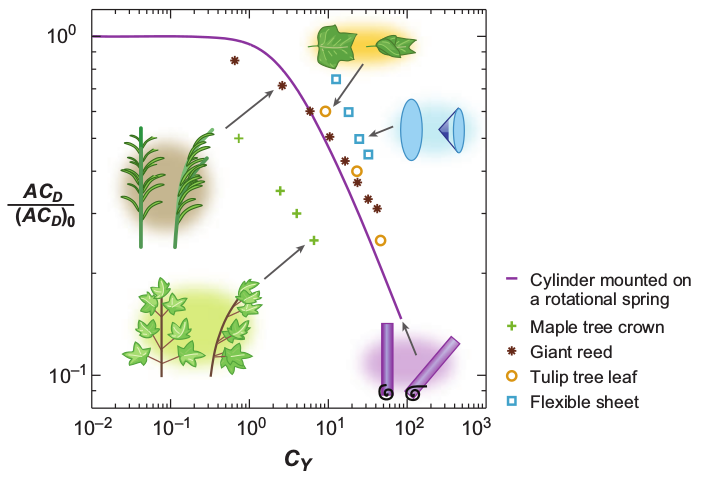
\includegraphics[width=0.7\linewidth]{chapter_1/cy_cd}
	\caption{The effect of the Cauchy number $C_Y$ on the drag reduction are presented in the figure. The drag reduction has been represented as the ration between the frontal area $A$ and the drag coefficient $C_D$ at static condition (subscript $0$) and the dynamic condition (no subscript). Image from \citet{de2008effects}}
	\label{fig:cycd}
\end{figure}

The overall reconfiguration of the permeable medium can lead to pressure recovery and a wake regularization applied when applied to a bluff body, as the experiments by \citet{gosselin2011drag} shows.

Another non-dimensional number to mention is the \textit{reduced velocity}, it can be derived form the previous ones:
$$ U_R = \sqrt{C_Y s / m^*},$$
this number is used dealing with vortex induced vibration of slender structures; when is near to one dynamical coupling between the fluid and the structure is expected, such as resonance or lock-in phenomena.

Canopies can also help to prevent separation in presence of adverse pressure gradients, \citet{belcher2012wind} show an analysis of the flow over an hill covered with canopies using either numerical and experimental data; the authors show how the permeable layer can present a re-circulation region inside the canopy in the decreasing slope side of the hill, this zone move the separation away from the flow over the hill to the internal structure of the canopy.
%In this sense when we look at the "global" hill (ground and canopy layer) the reversed flow typical of this geometry is not present.

Is important to pinpoint that the above results are restricted to fibrous or slender structure, and they cannot be extrapolated in general for different porous structure and shapes, even though similar mechanism are expected.

The research on canopy flow embrace a wide range of configurations and this makes very difficult the comparison of the results since most of the authors use very different models in a lot of various regimes of velocities using flexible structure with very different shapes.
Even if experiments are easier to find, like \citet{segalini2011experimental}, \citet{segalini2013scaling}, \citet{maza2013coupled}, \citet{barsu2016drag}, \citet{alvarado2017nature}, there is no quantitatively mathematical model established for the fluid and structure equations and almost all the models available rely on empirical correlations that fit the data in each different application.


\section{Models for flows through porous surfaces}

In this section we want to show some insight of the various models characteristic flow through poroelastic layers.
In order to be as clear as possible we have taken as example a very simple geometry to sketch the problem; the flow over a wall that include flexible multiple filaments. 
This simple geometrical configuration still has all the characteristic and difficulties of more interesting applications, such as a bluff body with a poroelastic layer.

\begin{figure}[h]
	\centering
	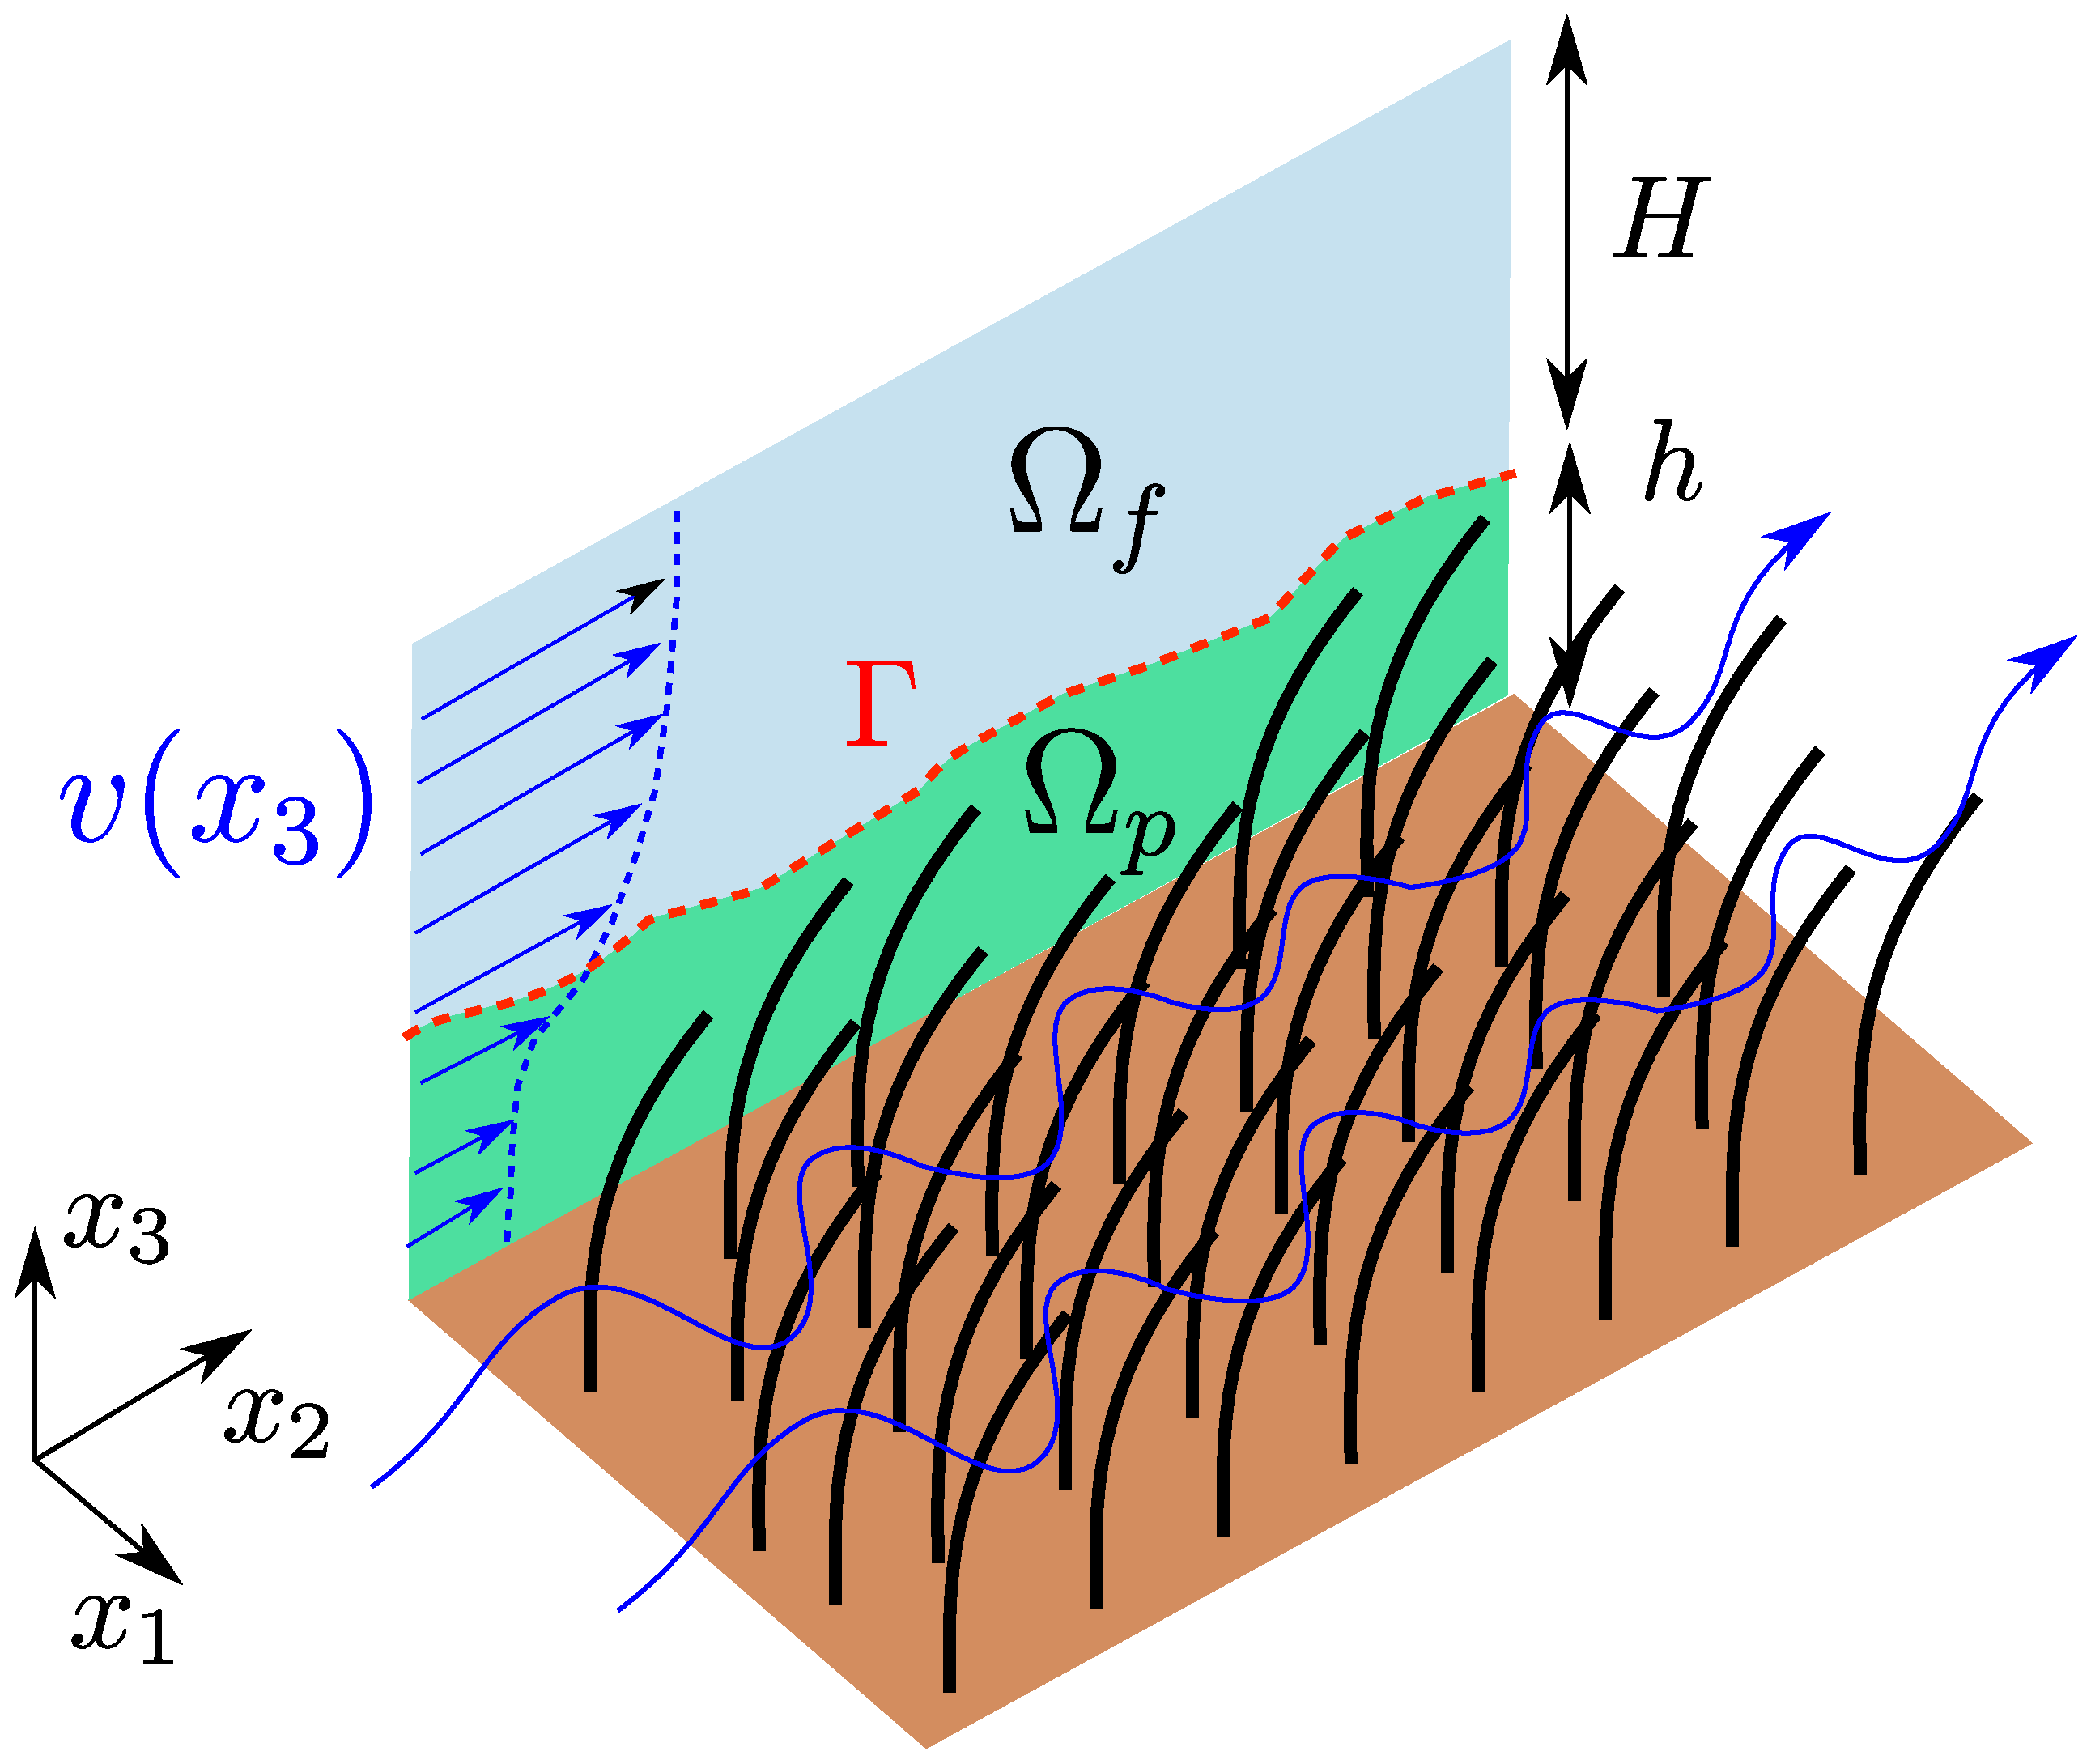
\includegraphics[width=0.7\linewidth]{chapter_1/problem_schema}
	\caption{Sketch of the fully developed flow over a poroelastic surface made of multiple filaments.}
	\label{fig:schema_problem}
\end{figure}

The figure \ref{fig:schema_problem} show a graphical schema of such flow; the main fluid direction is aligned with the $x_2$ axis and the projection of velocity stream-wise component is shown in the plane $x_2 - x_3$.
Such flow can bend the filaments and, of course, go by their ensemble.
The hypothetical surface that envelop all the filaments lid ($\Gamma$), defines the limit between the flow without obstacle ($\Omega_{f}$) and the one inside the poroelastic medium ($\Omega_{p}$), their projection are shown in the  $x_2 - x_3$ plane.

In order to computationally solve this problem there are some key points to address:
\begin{itemize}
	\item Length scales: the flow present interaction at multiple scales. The flow can develop Kelvin–Helmholtz type instabilities on the interface (of size $h$) and they can even penetrate inside the medium and brake up to very small scales eddies. In order to resolve this complex dynamic one should use a very fine numerical mesh (highly computational expensive) or came up with a model (like in the context of turbulence modeling).
	Turbulence dynamic can be also problematic; the hypothesis that pore size eddies can exist deep inside the porous medium is still at debate in the community.
	How to deal with such small scale dynamic and/or find a model is not an easy task.
	
	\item Compliance (fluid structure interaction): if the filaments are flexible, they can bend and swing due to the fluid impact on them.
	We have to take into account a mechanical solid model for the filaments (for example a the Bernoulli beam), including also the computation of energy that the swing motion will re-inject inside the fluid.
	This two-way coupling could also be really computational expensive in presence of a large number of filaments, and also, if the flexibility is important one should in principle take into account the contact and repulsion between the fibers.
	If the porous medium has more complicated shape (like the scales in the butterfly wing) came out with a simplified model for the solid dynamic is even more difficult and the use of a general FEA discretization is probably a necessity (at it will increase the computational cost of the problem).
	Another approach consist of consider a "rheology" model for the medium, for example treat it like a porous medium that have elastic properties as an ensemble.
	Such models are applicable only to porous media where the solid inclusion are connected to each other; in principle they are convenient, computational speaking, but their mathematical description can be difficult.
	
	\item Anisotropy: the model used should be capable of treats permeable surfaces that have different responses when stressed in different directions. For example the geometrical disposition and/or the mechanical properties of the medium can be non-homogeneous, so it will be more permeable in one direction and show a preferential flow path.
\end{itemize}

\citet{dupont2010modelling} had performed a LES simulation introducing a two way coupling for the fluid-structure interaction problem, they validate their code with video recording of a similar experiment and the frequency measurements of the Kelvin–Helmholtz instabilities at the interface agrees very well.
The authors haven't specified the computational configuration used but they have mentioned an important high performance computing center in the acknowledgment which made us suppose that the computational power involved were substantial.
Recently also in \citet{marjoribanks2017does} a similar approach has been used.

Some other examples that solve the full coupled problem directly are in \citet{pinelli2017pelskin}, \citet{favier2017pelskin}, \citet{revell2017pelskin} but in this case the number of filaments is small and so they can be though more as isolated filaments rather that a poroelastic medium.

Due to the computationally expensiveness of solving the problem directly, the scientific community has came out with different approaches that treat the porous domain with a generalized model that do not resolve the fine scale inside the filaments but instead express them as a function of the larger length scales present in the fluid domain $\Omega_{f}$.

These are called homogenization approaches and the key point in such methods are:
\begin{itemize}
	\item The division of the overall domain in two different parts: the fluid domain $\Omega_{f}$ and the porous domain $\Omega_{p}$
	\item Two different fluid models are solved in the two domains, in $\Omega_{f}$ the Naver-Stokes equations for incompressible Newtonian fluids are solved. In the porous part there are a number of different models that adds source terms in the former equations to take into account the presence of the porous medium.
	\item The two domains should be coupled together with a boundary condition at the interface or a special treatment for the equation in the transition region.
	\item A model for the dynamic of the solid porous part, it can model the structures directly or with an averaged rheology model.
\end{itemize}

The key points showed above will be extensively expanded, in chapter \ref{ch:vans}, for the homogenization method chosen in this thesis.
However in the next sections the two main branches in literature, that takes into account the presence of a porous medium layer, will be summarized in order to give a panoramic on all the possible choices.


\subsection{Isotropic drag models}
\label{sec:canopy_eq}

In the case of flow through vegetation (canopy flows) it is common to use an isotropic drag model (the drag is equal in the three principal directions of the medium) for parameterize the resistance of the canopy.
The drag can be a function of the wall normal direction and but in most of the application is taken as a constant.
The isotropic hypothesis can be correct in case of dense vegetation; even if the vertical component of the resistance should be smaller.
However since this models are mostly applied in channel problems where the mean flow is mostly stream-wise, the resistance in the vertical direction can be approximated in this manner; but in application where the transpiration of the interface is important (wake control of bluff body) the isotropic drag model is certainty, not the most adequate.

The drag resistance is included in the Navier-Stokes equations as a sink of momentum \eqref{eq:mom_cd}.

\begin{equation}
\derp{\vb}{t} + \vb \cdot \nabla \vb = -\frac{1}{\rho_{\beta}} \nabla \pb + \nub \nabla^2 -C_D a |\vb| \vb, 
\label{eq:mom_cd}
\end{equation}

The sink term is quadratic in the velocity but there is some evidence that the reconfiguration phenomena can change this relationship as a consequence of the drag reduction \citet{gosselin2011drag}, \citet{alvarado2017nature}.

The sink term also includes the parameter $a$ that is the frontal area per unit volume of the vegetation, this parameter is an expression of the porosity of the medium.

For our point of view this approach lack of strong mathematical formalism, from which one should be able to derive all the additional terms of the equations; as a consequence, this method heavily relies on empirical relations.
The other problem is that the isotropic hypothesis rule out the possibility to model the anisotropic nature of most of the surfaces in which we are interested (as equation \eqref{eq:max_dr} suggest the difference in the permeability in different directions can be important for the drag reduction).

But in the field of flow through vegetation some authors have successfully used this approach, for example \citet{maza2013coupled}, \citet{maza2015tsunami} use it to study wave attenuation and \citet{ghisalberti2004limited}, \citet{battiato2014single} develops simple models for the 2D mean flow over a canopy.


\subsection{Homogenization models}

In this section we want to introduce the most used approach to derive the equations valid in the porous domain.
The fundamental idea is to construct a micro-scale model, either for the fluid as for the solid, and then derive the macro-scale equations using some averaging operator over the micro-scale.

The two most used homogenization methods are the \textit{Volume Averaging} method \citet{whitaker2013method}, and the \textit{Multiple Scales} method \citet{mei2010homogenization}; they can be more broadly classified as perturbations methods. 
The key differences and the main results retrieved using this approaches will be presented in the following.


\subsubsection{Volume Averaging}
\label{sec:vans}

The method of Volume Averaging has been developed to threat transport equation in porous media applications; in this case the presence of two different length scales is obvious as in figure \ref{fig:porsystem}.
	
	\begin{figure}[h]
		\centering
		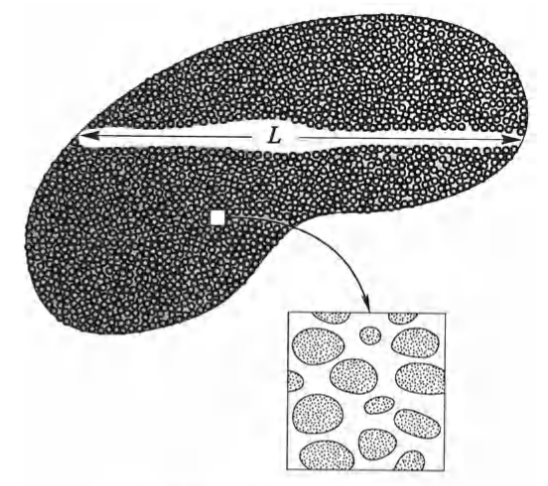
\includegraphics[width=0.5\linewidth]{chapter_1/por_system}
		\caption{Schematics os a porous media system of size $L$, with a zoom on the microscopic structure and its scale $\ell$}
		\label{fig:porsystem}
	\end{figure}

The core idea of the methods is to firstly define an average operator as \eqref{eq:avg_intrinsic_intro}; in this case the variable $\psi$ represent any vector or scalar variable in the system of equations that we want to homogenize, for Navier-Stokes it will be the velocity and the pressure.

\begin{equation}
\meani{\psi} = \dfrac{1}{\volb} \int_{V} \psi \, d \, V,
\label{eq:avg_intrinsic_intro}
\end{equation}

The average operator has the purpose to "scale up" the equation, in fact the second crucial step of the method is to decompose the variables as proposed by \citet{gray1975derivation}:

\begin{equation}
\psi =   \underbrace{ \meani{\psi} }_\text{O($L$)}  +  \underbrace{\tilde{\psi} }_\text{O($\ell$)},
\label{eq:vans_decomp}
\end{equation}

The \eqref{eq:vans_decomp} show how each variable can be decomposed in an averaged part that contains only spatial variation at the macro-scale $L$ and a \textit{fluctuation} part that contains only the micro-scale $\ell$ spatial variations.

The decomposition can be injected in the transport equations that we want to homogenize, and after some mathematical manipulation is possible to retrieve the new averaged equations that includes only variables of order O($L$).
Since this is the method chosen to develop our work, all the technical details will be detailed explained in the chapter \ref{ch:vans}.

To introduce briefly some other aspects on the method we will show as example, how to derive the homogenized version of the Stokes equation. The described problem is a  flow inside a rigid porous medium, as the one in figure \ref{fig:porsystem}.
The Stokes equation valid for the liquid phase, indicated with the $\beta$ subscript, read:

\begin{equation}
0 = -\dfrac{1}{\rho_{\beta}} \nabla \pb +\nub \nabla^2 \vb
\label{eq:stokes}
\end{equation} 

Here is important to pinpoint that the equation \eqref{eq:stokes} is valid only in the liquid phase and to solve it we have to consider a no-slip boundary condition at the interface with the solid phase, with the difficulties that came to define the complex structure of the solid inclusion.
Applying the Averaging Method, we can derive a homogeneous version of the \eqref{eq:stokes} that is valid in all the porous domain that include the two different phases, the solid and the liquid one.
The homogenized version of the last is the famous Darcy equation \eqref{eq:darcyeq}, \citet{whitaker1986flow}.

\begin{equation}
\vbmi = -\dfrac{\mathbf{K} \varepsilon}{\mub} \nabla \pbmi
\label{eq:darcyeq}
\end{equation} 

In the Darcy equation is possible to recognize two additional quantities that arise from the averaging procedure, the fist one is a scalar called porosity $\varepsilon$ that represent the ratio between the volume of the liquid present in a reference volume, over the total volume itself.
The second one is the tensor $\mathbf{K}$ called permeability, it express the resistance of the porous medium that affect the flow in its travel.
The term $\mathbf{K}$ play the same role as $C_D a$ in the isotropic drag model; but the main difference is that the permeability tensor can be computed directly from the geometry of the medium (see chapter \ref{ch:vans}) so it does not rely on empirical relations.
Also the tensorial nature of this terms permits us to model porous inclusion that are anisotropic.

Applications of the theory include: flow where inertial terms are not negligible \citet{whitaker1996forchheimer}, porous media with small deformations \citet{whitaker1986flow2}, and high deformations \citet{hussong2011continuum}, turbulent problems \citet{soulaine2014}, \citet{breugem2006influence}, interface between a permeable medium and a free flow \citet{beavers1967boundary}, multi-phase systems \citet{whitaker1973transport}, heat transfer \citet{carbonell1984heat}.

Is impossible to go into details in the derivation of equation for each specific problem but hope that the readers have understand the differences between this method and the isotropic drag model of the previous section.
%One of the greatest differences is the robustness that came from a mathematical formalism instead of an approach rely heavily on experimental closure terms.

\subsubsection{Multiple Scales}

The multiple scale method is similar to the previous one; and it has also been applied to similar problems in the context of porous media applications.

In this method we start with the assumption of scale separation between $\ell$ the micro-scale and $L$ the macro-scale.
The scale separation factor can be defined as $\epsilon = \ell/L \ll 1$.
Using the same examples as before we want to show the how to compute the homogenized version of the Stokes equation for fluid flow through a porous media.
We introduce the micro-scale and the macro-scale coordinates of the problem defined respectively as:
$$
 X_i = \dfrac{\tilde{x_i}}{L}, \quad   x_i = \dfrac{\tilde{x_i}}{\ell},
$$
where $x_i$ are the original eulerian coordinate of the problem.
Using the above separation factor is possible to expand the variables of the problem (pressure and velocity) into different magnitude orders (like a Taylor expansion) indicated as superscript:
$$
\psi(X_i, x_i) = \psi^{(0)}(X_i, x_i)  +\epsilon \psi^{(1)}(X_i, x_i) +\epsilon^2 \psi^{(2)}(X_i, x_i) +O(\epsilon^3),
$$
injecting this decomposition inside the equation \eqref{eq:stokes} is it possible to derive a set of system of equations for each order of the expansion.
It can be shown that analyzing each equation in the set we can retrieve the homogenized equation:

\begin{equation}
{v_i}^{(0)} = -K_{ij} \dfrac{\partial p^{(0)}}{\partial X_i}
\label{eq:darcy_ms}
\end{equation} 

In which either the pressure or the velocity fields appear only at the order zero, and the equation depends only on the macro-scale length.

The same permeability tensor $\mathbf{K}$ as before is retrieved, with the same definition and interpretation.
It is clear that for this example problem we end up with the same set of homogenized equation; what change are the starting hypotheses of the method and the mathematical development to compute them.

A full analysis of the dualism of the two approaches can be found in the work by \citet{davit2013homogenization}.

The multiple scale also has been used to study many other problems: inertial effects \citet{mei1991effect}, \citet{skjetne1999new}, coupling between a free fluid and a porous media \citet{mikelic2000interface}, porous media with small deformations \citet{auriault1977etude}, heat conduction in composites \citet{auriault1983effective}, rigid and moving permeable layers \citet{zampogna2016fluid}, \citet{ugis}, \citet{zampogna2017pelskin}.

Is also worth mention another homogenization based method called \textit{Mixture Theory}.
It is based on a similar approach as the previous ones and  \citet{rajagopal2007hierarchy} have shown that it is possible to retrieve the same equation as the previous two methods in case of porous media flow.


\section{Stability of flow over permeable surfaces}
\label{sec:stability}

Flows through submerged aquatic plants exhibit large scale vortices at the top of the vegetation,
advecting along the flow direction and causing a periodic waving of the plants, referred to as
monami (if the fluid is air) and honami (in case of water) \citet{inoue1955studies}, \citet{ackerman1993reduced}.
The effect of the onset of the monami is depicted in figure \ref{fig:monai_evol}.

\begin{figure}[h]
	\centering
	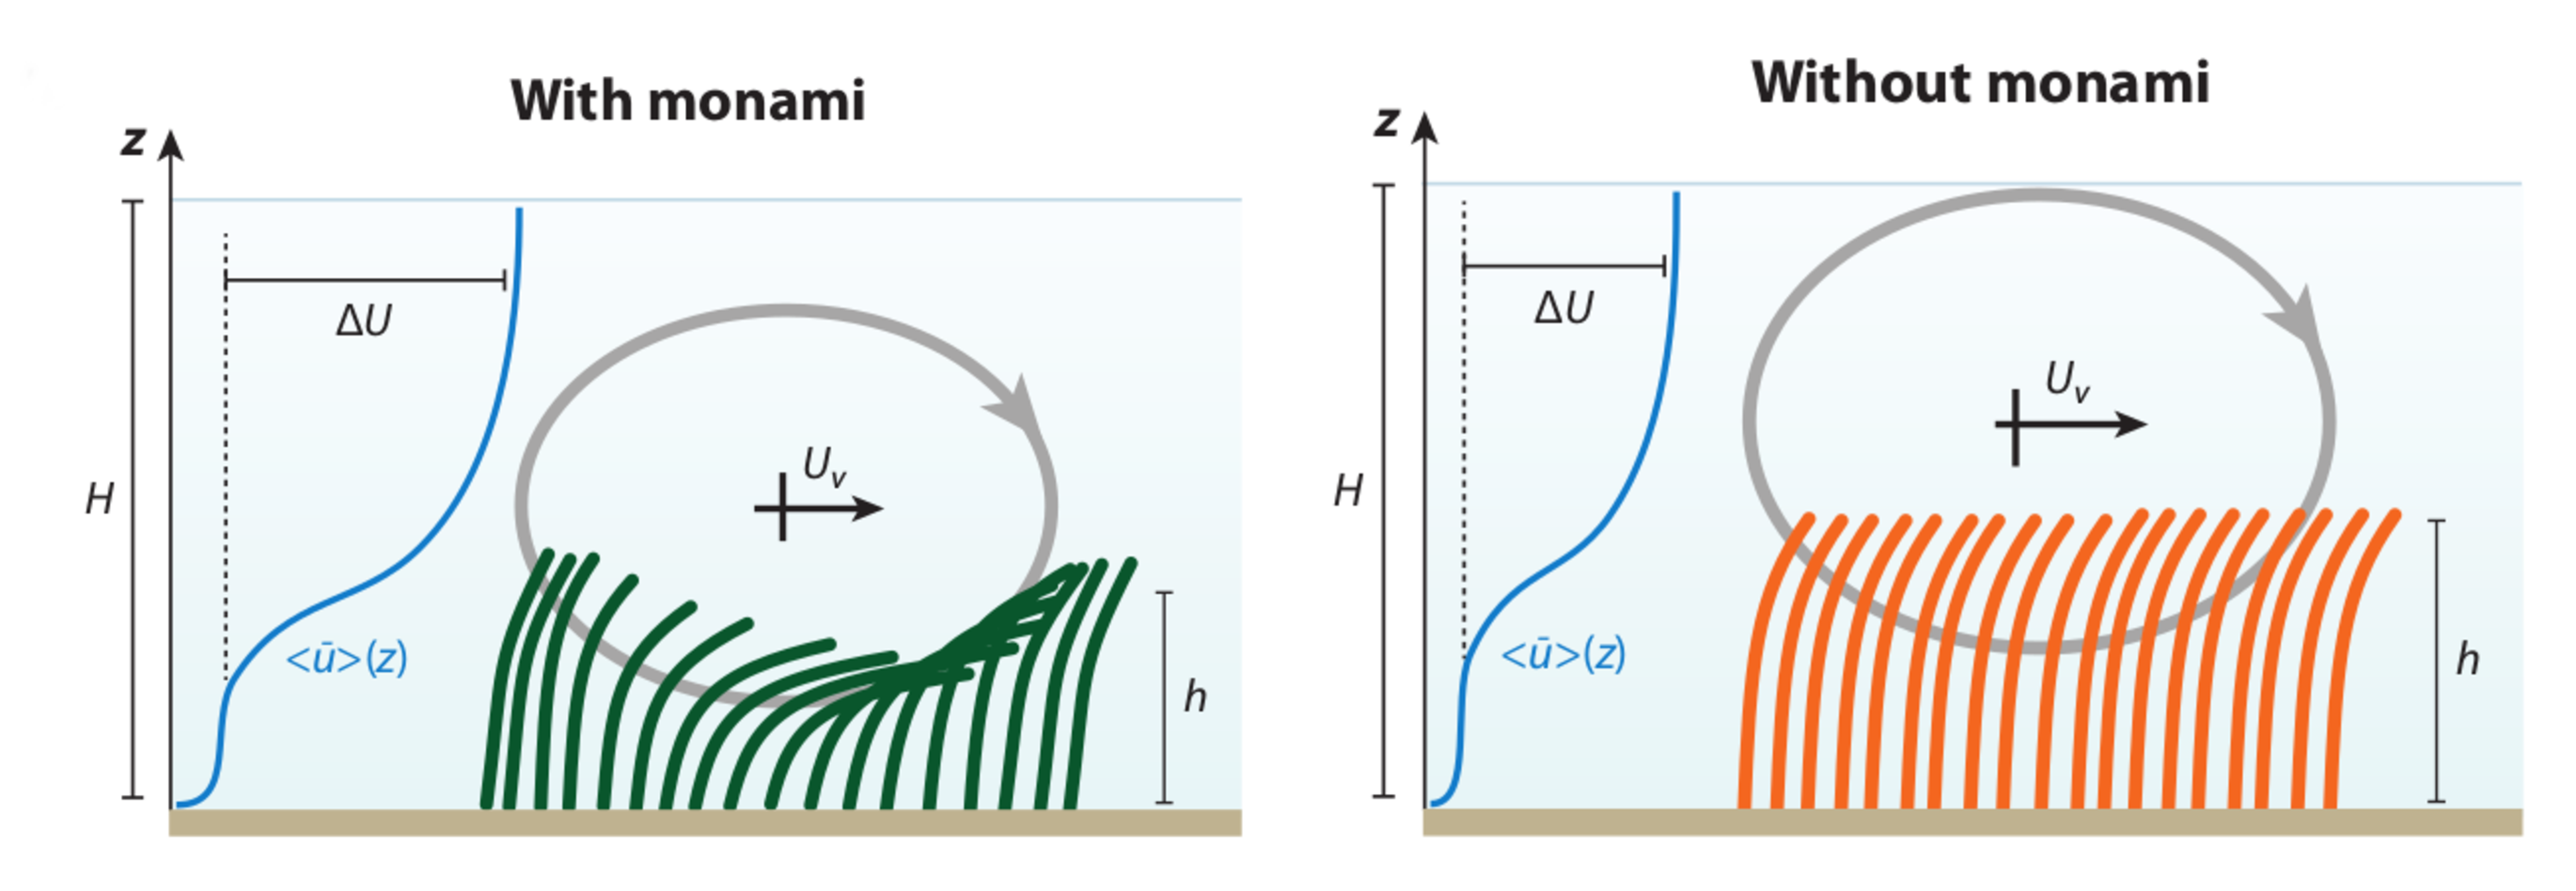
\includegraphics[width=1\linewidth]{chapter_1/monami}
	\caption{Left: when the drag of the canopy is high enough it generates canopy-scale vortices by Kelvin-Helmholtz instability. These vortices may interact with the flexible vegetation and generate a waving motion called monami. Right: when this interaction is too weak, the canopy will only bend. Image from \citet{nepf2012flow}}
	\label{fig:monami}
\end{figure}

Vortices arise from the nonlinear amplification of a Kelvin-Helmholtz instability mode, related to the presence of an inflection point in the base flow profile \citet{asaeda2005morphological}; the profile itself is inflectional because the fluid is slowed down by the drag exerted by the canopy, whose modeling has recently been addressed \citet{py2004mixing}, \citet{singh2016linear},  \citet{zampogna2016instability}, \citet{tilton2008linear}.
The correct prediction of the onset and characteristics of the Kelvin-Helmholtz instability is important for assessing the effects of turbulence \citet{finnigan2000turbulence}, \citet{jimenez2001turbulent} in particular to:

\begin{itemize}
	\item understand how the vertical exchange of momentum occurs \citet{ikeda1996three}
	\item clarify how the transport of $\text{CO}_2$ and dissolved nutrients or sediments takes place. This exchange takes place between the
	obstructed vegetation flow and the free overflow motion \citet{gambi1990flume}, \citet{eckman1987role}, \citet{grizzle1996hydrodynamically}
	\item assess the changes in the morphology of the vegetation in inland or coastal wetlands in
	response to continuous periodic forcing \citet{asaeda2005morphological}, \citet{patil2010characteristics}
\end{itemize}

One of the possible approach to study how and when these instability develops is the linear instability analysis; in the following section we will briefly introduce the key assumption and simplifications of the method over other possible choices, and in the next section some results in the context of permeable surfaces will be presented.


\subsection{Stability theory generalities}

Stability theory in general covers the modeling of transition of fluids systems towards not stables states and at least turbulence.
In its most basic form the theory gives us a fast and robust method to compute the frequency and grow rate of the unstable modes, if there is any, in the base flow.

The linear stability relies on the decomposition of the flow variables $\mathbf{q}$ into a steady-state part $\overline{\mathbf{q}}$ called base flow, and an unsteady part $\widetilde{\mathbf{q}}$:

$$ \mathbf{q} (\mathbf{x},t)= \overline{\mathbf{q}} (\mathbf{x}) + \eta \widetilde{\mathbf{q}} (\mathbf{x},t) $$

here $\eta$ is a small amplitude parameter.
Than the unsteady part is simplified by the hypothesis to have a general wave form:
$$  \widetilde{\mathbf{q}} =  \widehat{\mathbf{q}} e^{i\Theta} $$

where the $\widehat{\mathbf{q}}$ is the amplitude and the $\Theta$ is the phase of the perturbation.
The choice made to determine the time and space dependence of either the phase function and the amplitude determine a certain hierarchy inside the stability theories; the figure \ref{fig:table} below show the main choice made in the literature and the theory that derive from it:

\begin{figure}[h]
	\centering
	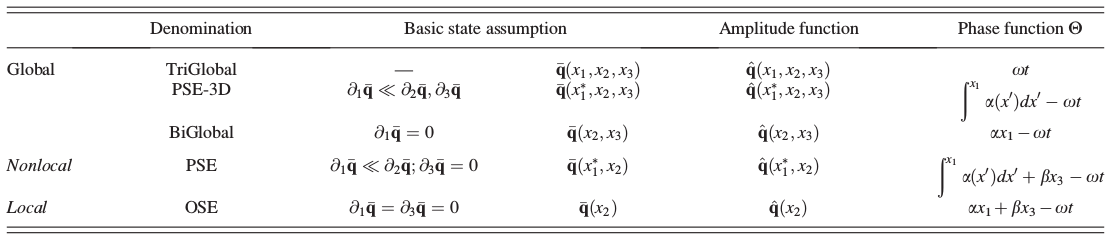
\includegraphics[width=1\linewidth]{chapter_1/table}
	\caption{Classification of modal linear stability theories. Table reported from \citet{juniper2014modal}}
	\label{fig:table}
\end{figure}
 
In our case we have limits our study in the linear stability theory (LST), that is a local approach based on mode decomposition.
In the LST we made the hypothesis that the amplitude and the base flow depend only on the wall normal spatial coordinate (parallel flow) and the phase function take into account the periodicity in time and in the stream-wise and cross-flow directions.
The complete formulation is in the following equation:
 $$  \widetilde{\mathbf{q}}(\mathbf{x},t) =  \widehat{\mathbf{q}}(x_2) e^{i(\alpha x_1 + \beta x_3 - \omega t)}  $$ 
where:
\begin{itemize}
	\item $\alpha$ is the stream-wise wave-number
	\item $\beta$ is the cross-flow wave-number
	\item $\omega$ is the wave phase
\end{itemize}

Casting this form for the pressure and velocity inside the Navier-Stokes equation and neglecting the second order terms ($\eta^2$) the equations became linear and  describes the evolution of the perturbations, taking the base flow as an input of the problem.
If we make the choice to impose that the $\alpha$ and $\beta$ wave-numbers are real and $\omega$ is complex the problem became a generalized eigenvalue one.
The above choice is made in order to study the stability of the perturbation in their time evolution and is know as \textit{temporal stability}.
The generalized eigenvalue problem for the wave phase has the form:

$$ A \widehat{\mathbf{q}} =  \omega B\widehat{\mathbf{q}} $$

and the solution gives use the frequency (real part of the eigenvalues) and the grow rate (imaginary part) of the perturbation modes (eigenvectors) of the flow.

The above introduction of the method is quite condensed, however, a lot of literature has been developed in these years on the subject, like: \citet{juniper2014modal}, \citet{criminale2003theory}, \citet{schmid2012stability}; the problem has also been extensively studied in his computational aspect \citet{canuto1988spectral}.

\subsubsection{Monami/Honami and Kelvin-Helmholtz rolls}

We have already pinpoint that the above framework for the stability problem has been applied in some porous media flow (canopy) configurations, also including the vegetation movement.
Because of the flexibility of the vegetation, some theoretical studies have focused on the
modeling of the stems of the aquatic plants and their displacement in response to the forcing by the
water flow \citet{py2004mixing}, \citet{patil2010characteristics}, \citet{gosselin2009destabilising}, \citet{py2006frequency}.

It has been studied in \citet{finnigan2000turbulence} that these large coherent structures control turbulence dynamics over the canopy. 
Movements of the latter generate sweeps (and ejections) of fluids that generates the counter-rotating stream-wise eddy evolving as Kelvin-Helmholtz rolls.
This picture of this complex evolution rich in vortex dynamics is shown in figure \ref{fig:monai_evol}.

\begin{figure}[h]
	\centering
	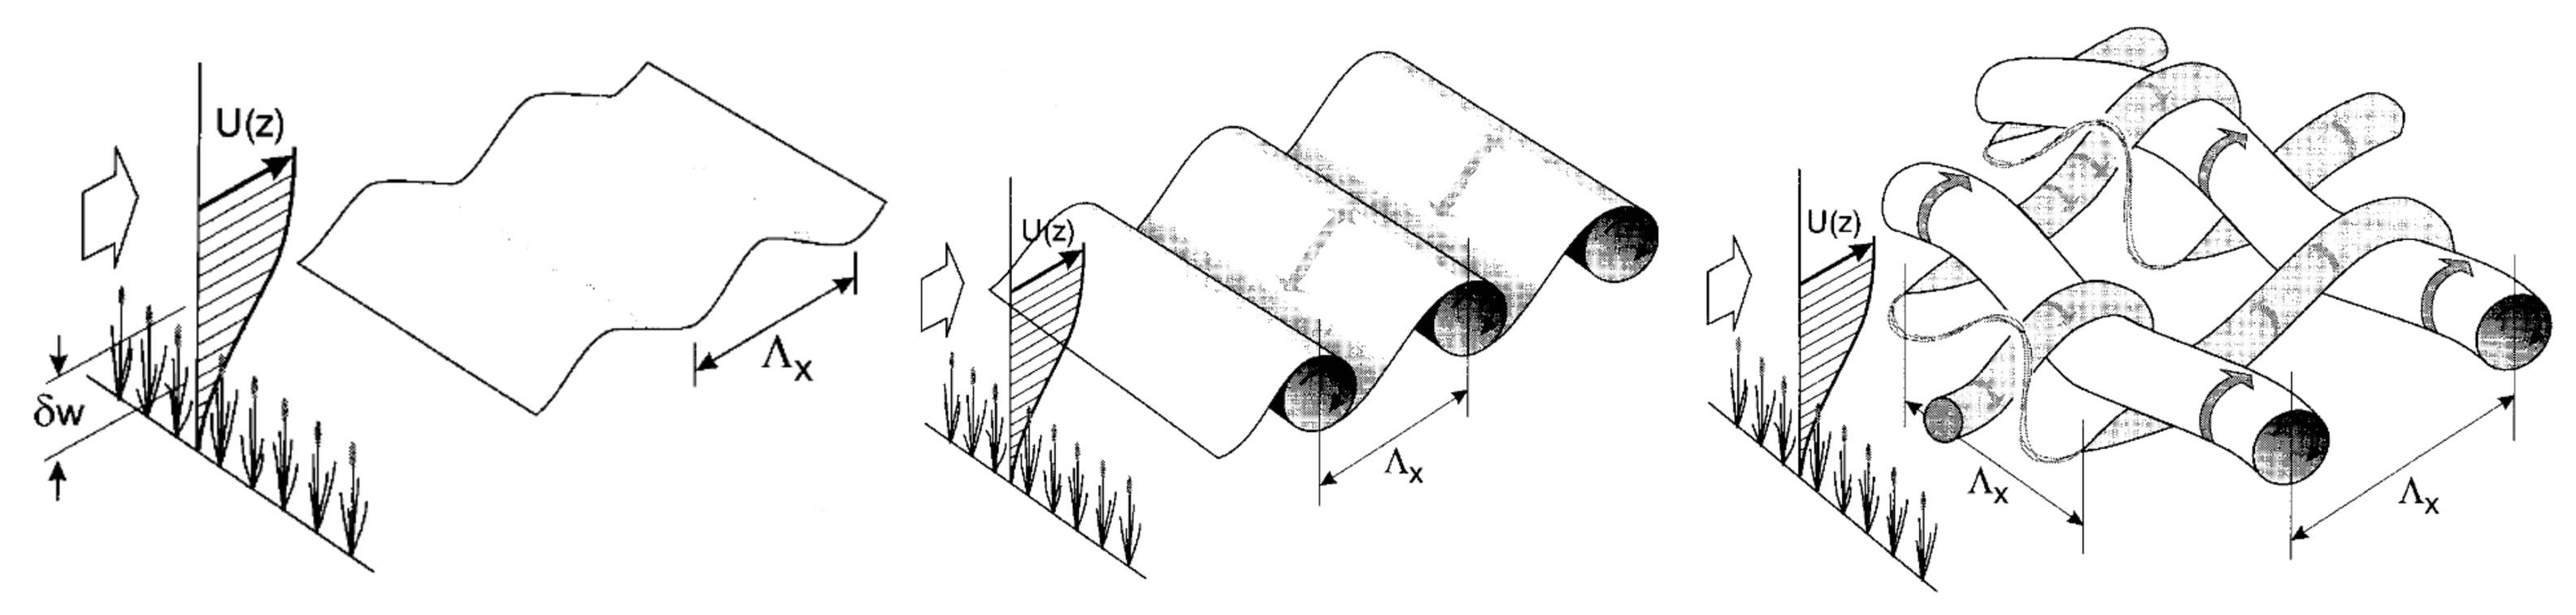
\includegraphics[width=1\linewidth]{chapter_1/finn}
	\caption{Left: first emergence of the Kelvin-Helmholtz instability here the grow rate is proportional to the shear magnitude at the inflection point. Center: the instability evolves in rollers of consisting in high vorticity that are spaced with a similar wave-length $\Lambda_x$ as the previous stage.  Right: secondary instabilities in the rollers lead to their kinking and pairing, coherent structures shows up in the transverse and stream-wise dimensions. Image from \citet{finnigan2000turbulence}}
	\label{fig:monai_evol}
\end{figure}


However, Kelvin-Helmholtz vortices occur whether or not the plants bend and to ascertain causes and effects to first order it is acceptable to focus on rigid porous structures.
The flow over and through a submerged array of rigid, cylindrical pillars has been the basis of the approach by \citet{ghisalberti2002mixing}, \citet{ghisalberti2004limited}, \citet{ghisalberti2005mass} who have conducted a series of careful experiments; their results have often been used by fluid dynamicists to put forth and test theoretical hypotheses to predict the frequency and
wavelength of the large scale vortical motion, for a variety of conditions.
The configuration studied consists of a regular grid of rigid pillars, orthogonal to the surface, of identical height $h$; in some
of the theoretical models proposed to analyze the stability of this system, the Rayleigh equation is
used throughout the water channel, with or without a drag term in correspondence of the canopy \citet{raupach1996coherent}, \citet{py2004mixing}, \citet{singh2016linear}, \citet{zampogna2016instability} have recently demonstrated that the addition of a drag term through the vegetation reduces the amplification factor of the Kelvin-Helmholtz instability throughout the whole range of wave-numbers and increases mildly the wavelength of the fastest growing mode.
In the chapter \ref{ch:stability} we will also study how perturbation of base flow affects the predicted amplification factor and wave-length, also we will test the difference between the isotropic drag model and the tensorial approach in order to show which is the most robust approach for stability computations.





